%=========================================================
%  RTL Verification Methods
%=========================================================
\section{RTL Verification Methods}


%=========================================================
%  Vector Simulation
%=========================================================
\subsection{Vector Simulation}

A directory named “mmRISC-1/simulation/modelsim/mmRISC\_Simulation” contains a sample set of vector simulation environments. The directory name "modelsim" refers to the predecessor application of Questa for logic simulation.

\begin{description}

    \item[(a) Common Preparation (Do Once)]\mbox{}\\
Before you try a simulation, please build "tools/hex2v.c" and "tools/hex2mif.c" once by using the following command, and add the locations of the generated executable binaries "hex2v" and "hex2mif" to the environment variable \$PATH. If your environment is Windows, use MinGW-64 or other appropriate compiling tools for standard C programs.\\

\texttt{\$ gcc -o hex2v hex2v.c}\\
\texttt{\$ gcc -o hex2mif hex2mif.c}\\

    \item[(b) Preparation of Script Command for Questa]\mbox{} \\
Please edit a command script file "sim\_TOP.do" if necessary. The default script instructs the following operations.\\

- To convert an Intel Hex binary program code “*.hex” to "rom.memh", which initializes an instruction RAM by \texttt{\$readmemh()} in the RTL code, use the command “hex2v” prepared above. Please edit the binary code file name if you want to change the codes to be stored in the instruction RAM.

- To compile each RTL file for verification by the command “vlog”. Please edit the RTL file list if you change the structure of RTL files.

- To launch the Simulator by the command “vsim”.

- To add Signals to display in the Wave Window by using Questa internal command “add wave”. Please edit the command list if you want to change the waveform display.

- To start Logic Simulation by the Questa internal command “run”.

- The RTL codes of the Instruction RAM and the Data RAM infer FPGA Block RAM IP and do not explicitly include the FPGA IP. If you want to include FPGA Block RAM IP with initialized data for the Instruction RAM, please add the option "+define+FPGA" in the vlog command. This macro switches ram.v to ram\_fpga.v for the Instruction RAM (RAM1) in the chip\_top layer. The ram\_fpga.v refers to the FPGA IP of RAM128KB\_DP.v stored in the directory “fpga”. The initialization data is specified by RAM128KB\_DP.mif which can be generated by using the following command.\\

\texttt{\$ ./tools/hex2mif ***.hex >  RAM128KB\_DP.mif}\\

Note that the Block RAM is made by a 2-Port type because the AHB write data period is after the active period of the address and strobes.

    \item[(c) Preparation of RTL for Test Bench]\mbox{} \\
Please edit the RTL code of the test bench "tb\_TOP.v", if necessary. In the test bench, the following features are supported.\\

- Generation of Reset and Clock
- Instantiation of CHIP\_TOP\_WRAP (chip\_top\_wrap.v)
- Simulation Time Out (\textasciigrave TB\_STOP)
- Initialization of nodes in the Power-On-Reset circuit.
- Simulation Stop Condition (Both reaching the end of the stimulus or writing to a Memory at address = 0xfffffffc with wdata = 0xdeaddead)
- Dumping out instruction Decode Sequences to "dump.txt" (if \textasciigrave DUMP\_ID\_STAGE is defined)
- Tasks for JTAG/cJTAG  Access (JTAG Reset, Shift-In/Out IR/DR, DMI Write and Read); If \textasciigrave define ENABLE\_CJTAG is OFF, normal 4-wire JTAG operations are enabled. If it is ON, 2-wire cJTAG operations based on RISC-V OpenOCD are enabled. 
- Stimulus for the debugging operations (if \textasciigrave JTAG\_OPERATION is defined) : Read IDCODE, JTAG Reset, Debugger Command for Stop/Step/Run). 
- If you want to insert several wait cycles in Instruction RAM access and Data RAM access, define “\textasciigrave RAM\_WAIT” in “defines\_chip.v”. The wait cycles are determined by bit [3:2] of the access address in "ram.v" logic.
- If you want to implement multiple (four) harts in mmRISC-1 and let them intervene on bus access among them, define “\textasciigrave MULTI\_HART’ in "define\_chip.v". Each hart has different reset vector, but all harts fetch instruction codes from the same instruction RAM due to shadowed addressing.

    \item[(d) Run the Logic Simulation]\mbox{} \\
Set the current directory to "mmRISC-1/simulation/modelsim/mmRISC\_Simulation", and launch Questa by using the “vsim” command. In the Transcript window, enter the command "do sim\_TOP.do" to execute the command script.

    \item[(e) Check Waveforms and Dump File (if any)]\mbox{} \\
Hopefully, you will get successful results ! A Questa Screen Shot is shown in Figure \ref{fig:QUESTAWINDOW}.

\end{description}

\begin{figure}[H]
    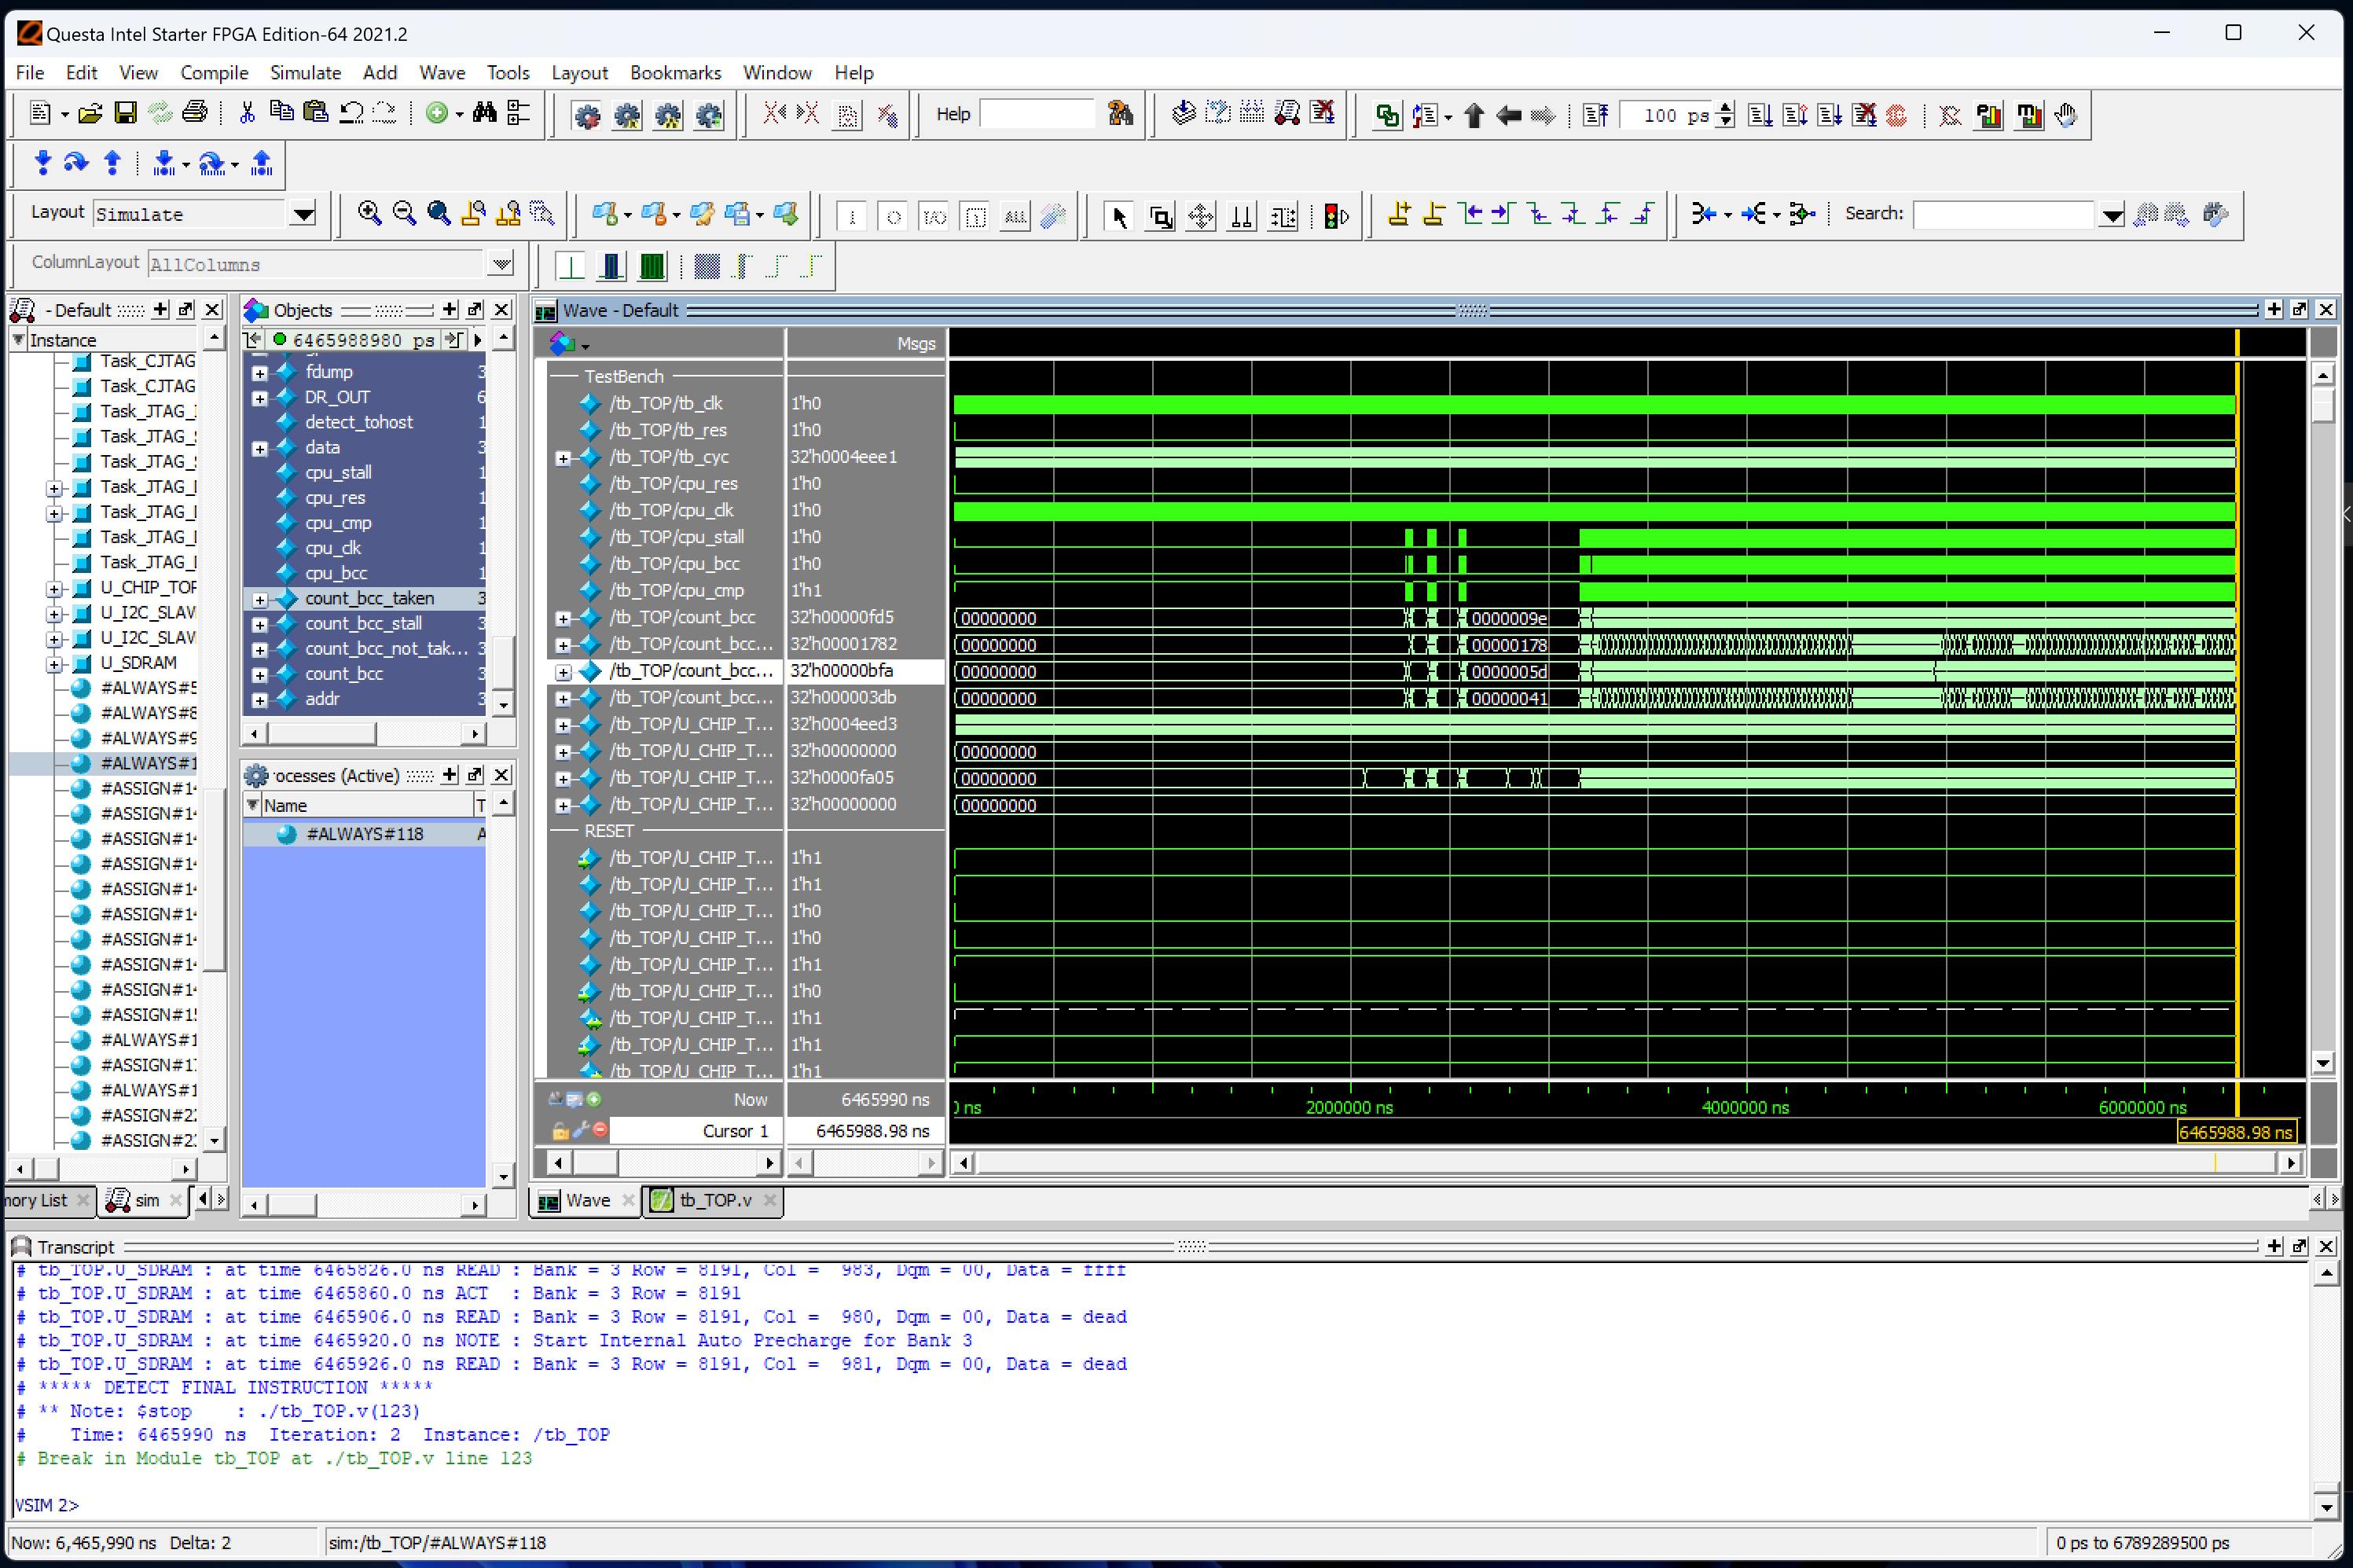
\includegraphics[width=0.8\columnwidth]{./Figure/QuestaWIndow.png}
    \caption{Questa Screen Shot}
    \label{fig:QUESTAWINDOW}
\end{figure}

%=========================================================
%  RISC-V Compliance Test "riscv-arch-test" for I/C/M/Zicsr/Zifence/Privileged
%=========================================================
\subsection{RISC-V Compliance Test "riscv-arch-test" \\ for ISA of I/C/M/Zicsr/Zifence/Privileged}

The directory "mmRISC-1/simulation/modelsim/riscv\_arch\_test" contains a sample set of compliance test resources for I/C/M/Zicsr/Zifence/Privileged instructions which are called "riscv-arch-test".

\begin{description}

    \item[(a) Preparation of "riscv-arch-test"]\mbox{}\\
The mmRISC-1 repository includes completed test binaries and signatures. However, if you want to prepare them by yourself, you need to install the RISC-V ISA Simulator "Spike" in advance. Then, you need to download "riscv-arch-test" from Github as shown in Table \ref{tb:DEVTOOLS}. After that, you need to follow its documentation and run the makefile to generate elf-binaries with disassembly lists. Next, you need to simulate them to generate expected signatures. You should place all the elf-binaries, disassembly lists and signatures under the directory "riscv-arch-test/work/rv32i\_m/*" and classify them by each ISA group. Finally, you should move to the directory \seqsplit{"riscv-arch-test" under the directory "mmRISC-1/simulation/modelsim/riscv\_arch\_test"}.   

    \item[(b) Running Simulations]\mbox{}\\
A python script "do\_riscv\_arch\_test.py" is prepared to execute the test automatically. It simulates the mmRISC-1 Tiny SoC with four different settings: (1) No RAM Wait Cycles + 1 Hart, (2) No RAM Wait Cycles + 4 Harts, (3) With RAM Wait Cycles + 1 Hart, and (4) With RAM Wait Cycles + 4 Harts. It takes each instruction sequence binary (elf) from “riscv-arch-test/riscv-arch-test/work/rv32i\_m/*/*.elf”, and simulates it. Each program code stores signature data in the address range from <begin\_signature> to <end\_signature>, and stores 0x00000001 in the address <tohost> at the end of the program. These <*> parameters are available in the corresponding disassembly list “.objdump” for each binary code. After the simulation is finished, the RTL test bench writes the stored data from <begin\_signature> to <end\_signature> into the dump list file “dump.signature”. The python script then compares the dump with the prepared expected signatures. If they are identical, the python script proceeds to simulate the next program code. Otherwise, the python script terminates. You can see reports like those in Listing \ref{list:RISCVARCHTEST}.

\end{description}

\begin{lstlisting}[caption=Output of "riscv-arch-test", label=list:RISCVARCHTEST, captionpos=b,  language=, frame=single, basicstyle=\ttfamily\scriptsize]
====[Test 1]======[BUS_INTERVENTION_01]=================
./riscv-arch-test/work/rv32i_m/privilege/misalign-blt-01.elf
Dump Begin 32'h90002080
Dump End   32'h90002190
To Host    32'h90001000
====[Test 2]======[BUS_INTERVENTION_01]=================
./riscv-arch-test/work/rv32i_m/privilege/misalign-lh-01.elf
Dump Begin 32'h90002080
Dump End   32'h90002190
To Host    32'h90001000
====[Test 3]======[BUS_INTERVENTION_01]=================
./riscv-arch-test/work/rv32i_m/privilege/misalign-beq-01.elf
Dump Begin 32'h90002080
Dump End   32'h90002190
To Host    32'h90001000
====[Test 4]======[BUS_INTERVENTION_01]=================
./riscv-arch-test/work/rv32i_m/privilege/ecall.elf
Dump Begin 32'h90002070
Dump End   32'h90002090
To Host    32'h90001000
...
\end{lstlisting}

%=========================================================
%  RISC-V Unit Test "riscv-tests" including Atomic and Floating Point ISA
%=========================================================
\subsection{RISC-V Unit Test "riscv-tests" \\including Atomic and Floating Point ISA}

The directory "mmRISC-1/simulation/modelsim/riscv\_tests" contains a sample set of unit tests, called "riscv-tests", that includes Atomic and Floating Point ISA.

\begin{description}

    \item[(a) Preparation of "riscv\_tests"]\mbox{}\\
The mmRISC-1 repository includes completed test binaries. However, if you want to prepare them by yourself, you need to download "riscv-tests" from Github as shown in Table \ref{tb:DEVTOOLS}. After that, you need to follow its documentation and run the makefile to generate elf-binaries and disassemble lists. You should place all the elf-binaries and disassemble lists under the directory "riscv-tests/work/isa/*" and classify them by each ISA group. Finally, you should move to the directory "riscv-test" under the directory "mmRISC-1/simulation/modelsim/riscv\_tests".

    \item[(b) Running Simulations]\mbox{}\\
A python script "do\_riscv\_tests.py" is prepared to run the test automatically. It simulates mmRISC-1 Tiny SoC with four different settings: (1) No RAM Wait Cycles + 1 Hart, (2) No RAM Wait Cycles + 4 Harts, (3) With RAM Wait Cycles + 1 Hart, and (4) With RAM Wait Cycles + 4 Harts. It takes each instruction sequence binary (elf) from "riscv-tests/riscv-tests/work/isa/RV32*/*" and simulates it. In the script file, you need to specify the directory according to the ISA you want to verify. For example, specify RV32IMC directory for RV32IMC, RV32IMAC directory for RV32A, and RV32IMAFC directory for RV32F and RV32FC. Each program code stores 0x00000001 in address <tohost> at the success point of the program, or stores different data in address <tohost> if it fails. You can find the <tohost> parameter in the corresponding disassembly list "*.dump" for each binary code. After the simulation finishes, the RTL test bench writes 'result.txt" that shows "PASS" or "FAIL" as a text. The python script then checks the result text, and if it is PASS, it proceeds to simulate the next program code. Otherwise, it terminates. You can see a report like the one in Listing \ref{list:RISCVTESTS}.

\end{description}

\begin{lstlisting}[caption=Output of "riscv-tests", label=list:RISCVTESTS, captionpos=b,  language=, frame=single, basicstyle=\ttfamily\scriptsize]
====[Test 1]======[BUS_INTERVENTION_01]=================
./riscv-tests/work/isa/RV32IMFC/rv32uf-p-fcvt_w
To Host    32'h90001000
====[Test 2]======[BUS_INTERVENTION_01]=================
./riscv-tests/work/isa/RV32IMFC/rv32uf-p-fclass
To Host    32'h90001000
====[Test 3]======[BUS_INTERVENTION_01]=================
./riscv-tests/work/isa/RV32IMFC/rv32uf-p-fadd
To Host    32'h90001000
====[Test 4]======[BUS_INTERVENTION_01]=================
./riscv-tests/work/isa/RV32IMFC/rv32uf-p-ldst
To Host    32'h90001000
====[Test 5]======[BUS_INTERVENTION_01]=================
./riscv-tests/work/isa/RV32IMFC/rv32uf-p-move
To Host    32'h90001000
...
\end{lstlisting}




